\documentclass[tikz,border=12pt]{standalone}
\usepackage[T1]{fontenc}
\usepackage{lmodern,amsmath,amssymb}
\usetikzlibrary{arrows.meta,positioning}
\definecolor{ink}{HTML}{183444}
\definecolor{blue}{HTML}{1B6780}
\definecolor{amber}{HTML}{AD601A}
\definecolor{purple}{HTML}{785696}
\begin{document}
\hyphenpenalty=10000\exhyphenpenalty=10000
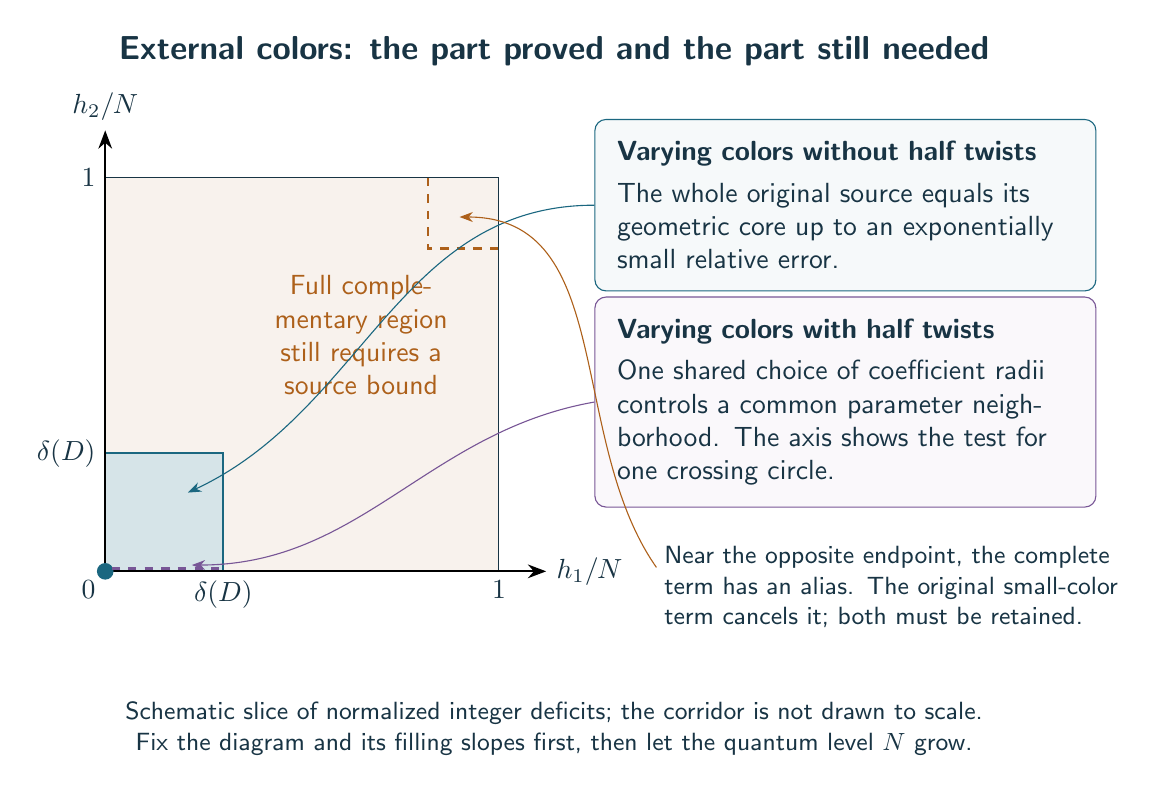
\begin{tikzpicture}[font=\sffamily,text=ink,>=Stealth]
 \node[font=\sffamily\large\bfseries] at (5.7,6.6)
 {External colors: the part proved and the part still needed};
 \fill[amber!8] (0,0) rectangle (5,5);
 \fill[blue!18] (0,0) rectangle (1.5,1.5);
 \draw[blue,thick] (0,1.5)--(1.5,1.5)--(1.5,0);
 \draw[ink,thin] (0,5)--(5,5)--(5,0);
 \draw[->,thick] (0,0)--(5.6,0) node[right] {$h_1/N$};
 \draw[->,thick] (0,0)--(0,5.6) node[above] {$h_2/N$};
 \node[below left] at (0,0) {$0$};
 \node[below] at (1.5,0) {$\delta(D)$};
 \node[below] at (5,0) {$1$};
 \node[left] at (0,1.5) {$\delta(D)$};
 \node[left] at (0,5) {$1$};
 \fill[blue] (0,0) circle (3pt);
 \draw[purple,very thick,dashed] (.08,.04)--(1.45,.04);
 \node[align=center,text width=3.2cm,amber] at (3.25,3.0)
 {Full complementary region\\still requires a source bound};
 \draw[amber,dashed,thick] (4.1,5)--(4.1,4.1)--(5,4.1);
 \node[draw=blue,fill=blue!4,rounded corners,align=left,
       text width=5.8cm,inner sep=8pt] (near) at (9.4,4.65)
 {\textbf{Varying colors without half twists}\\[3pt]
 The whole original source equals its geometric core up to an exponentially small relative error.};
 \draw[blue,->] (near.west) to[out=180,in=25] (1.05,1.0);
 \node[draw=purple,fill=purple!4,rounded corners,align=left,
       text width=5.8cm,inner sep=8pt] (signed) at (9.4,2.15)
 {\textbf{Varying colors with half twists}\\[3pt]
 One shared choice of coefficient radii controls a common parameter neighborhood. The axis shows the test for one crossing circle.};
 \draw[purple,->] (signed.west) to[out=190,in=0] (1.1,.08);
 \node[align=left,text width=5.8cm,font=\sffamily\small] at (10.0,-.2)
 {Near the opposite endpoint, the complete term has an alias. The original small-color term cancels it; both must be retained.};
 \draw[amber,->] (7.0,.05) to[out=125,in=0] (4.5,4.5);
 \node[align=center,text width=11.5cm,font=\sffamily\small] at (5.7,-2.0)
 {Schematic slice of normalized integer deficits; the corridor is not drawn to scale.\\
 Fix the diagram and its filling slopes first, then let the quantum level $N$ grow.};
\end{tikzpicture}
\end{document}
